% OpenAI Math Digest; follows the existing Schnell diagram style.
\documentclass[border=12pt]{standalone}
\def\pgfsysdriver{pgfsys-dvisvgm.def}
\usepackage[dvisvgm]{xcolor}
\usepackage{xeCJK}
\setCJKmainfont{HaranoAjiGothic-Regular.otf}[BoldFont=HaranoAjiGothic-Bold.otf]
\setCJKsansfont{HaranoAjiGothic-Regular.otf}[BoldFont=HaranoAjiGothic-Bold.otf]
\usepackage{amsmath,amssymb,tikz,lmodern}
\usetikzlibrary{arrows.meta,positioning,calc}
\renewcommand{\familydefault}{\sfdefault}
\definecolor{ink}{HTML}{25322F}
\definecolor{green}{HTML}{246657}
\definecolor{tint}{HTML}{EEF4F0}
\definecolor{soft}{HTML}{C6D2CC}
\definecolor{muted}{HTML}{52615B}
\definecolor{amber}{HTML}{866321}
\newif\ifJapanese
\newcommand{\Tx}[2]{\ifJapanese #1\else #2\fi}
\newcommand{\heading}[2]{{\color{green}\bfseries\Tx{#1}{#2}}\\[5pt]}
\newcommand{\refurl}[2]{\special{dvisvgm:raw <a xlink:href="#1" target="_blank" rel="noopener noreferrer">}{\color{green}\underline{\strut #2}}\special{dvisvgm:raw </a>}}
\newcommand{\R}[2]{\expandafter\refurl\expandafter{\csname source#1\endcsname}{#2}}
\tikzset{
 card/.style={draw=soft,fill=white,rounded corners=2pt,align=left,text=ink,font=\fontsize{10.5}{14}\selectfont,inner xsep=12pt,inner ysep=10pt,text width=14.4cm},
 result/.style={card,draw=green,fill=tint,line width=.9pt},
 reason/.style={align=left,text=muted,font=\fontsize{9}{12}\selectfont,inner sep=0pt,text width=12.65cm},
 edge/.style={-{Stealth[length=2.4mm]},draw=green,line width=1pt},
}
\newcommand{\flow}[3]{
 \coordinate (#2-from) at ($(#1.south)+(-6.9,0)$);
 \coordinate (#2-to) at ($(#2.north)+(-6.9,0)$);
 \draw[edge] (#2-from)--(#2-to);
 \node[reason,anchor=west] at ($(#2-from)!.5!(#2-to)+(.55,0)$) {#3};
}

\expandafter\def\csname sourceBS\endcsname{https://github.com/openai/math/blob/fd4aeeb2ee4fc729c18d98444fed42fd0529eeeb/preprints/B-semiampleness-for-compact-log-smooth-Kahler-fibrations-September-10-2026/paper.pdf}
\expandafter\def\csname sourceBFMT\endcsname{https://arxiv.org/pdf/2508.19215v2}
\expandafter\def\csname sourceFF\endcsname{https://arxiv.org/pdf/2304.00672v3}
\expandafter\def\csname sourceMWWZ\endcsname{https://arxiv.org/pdf/2506.23218v1}
\expandafter\def\csname sourceToma\endcsname{https://arxiv.org/pdf/1103.5835v3}
\Japanesetrue
\begin{document}
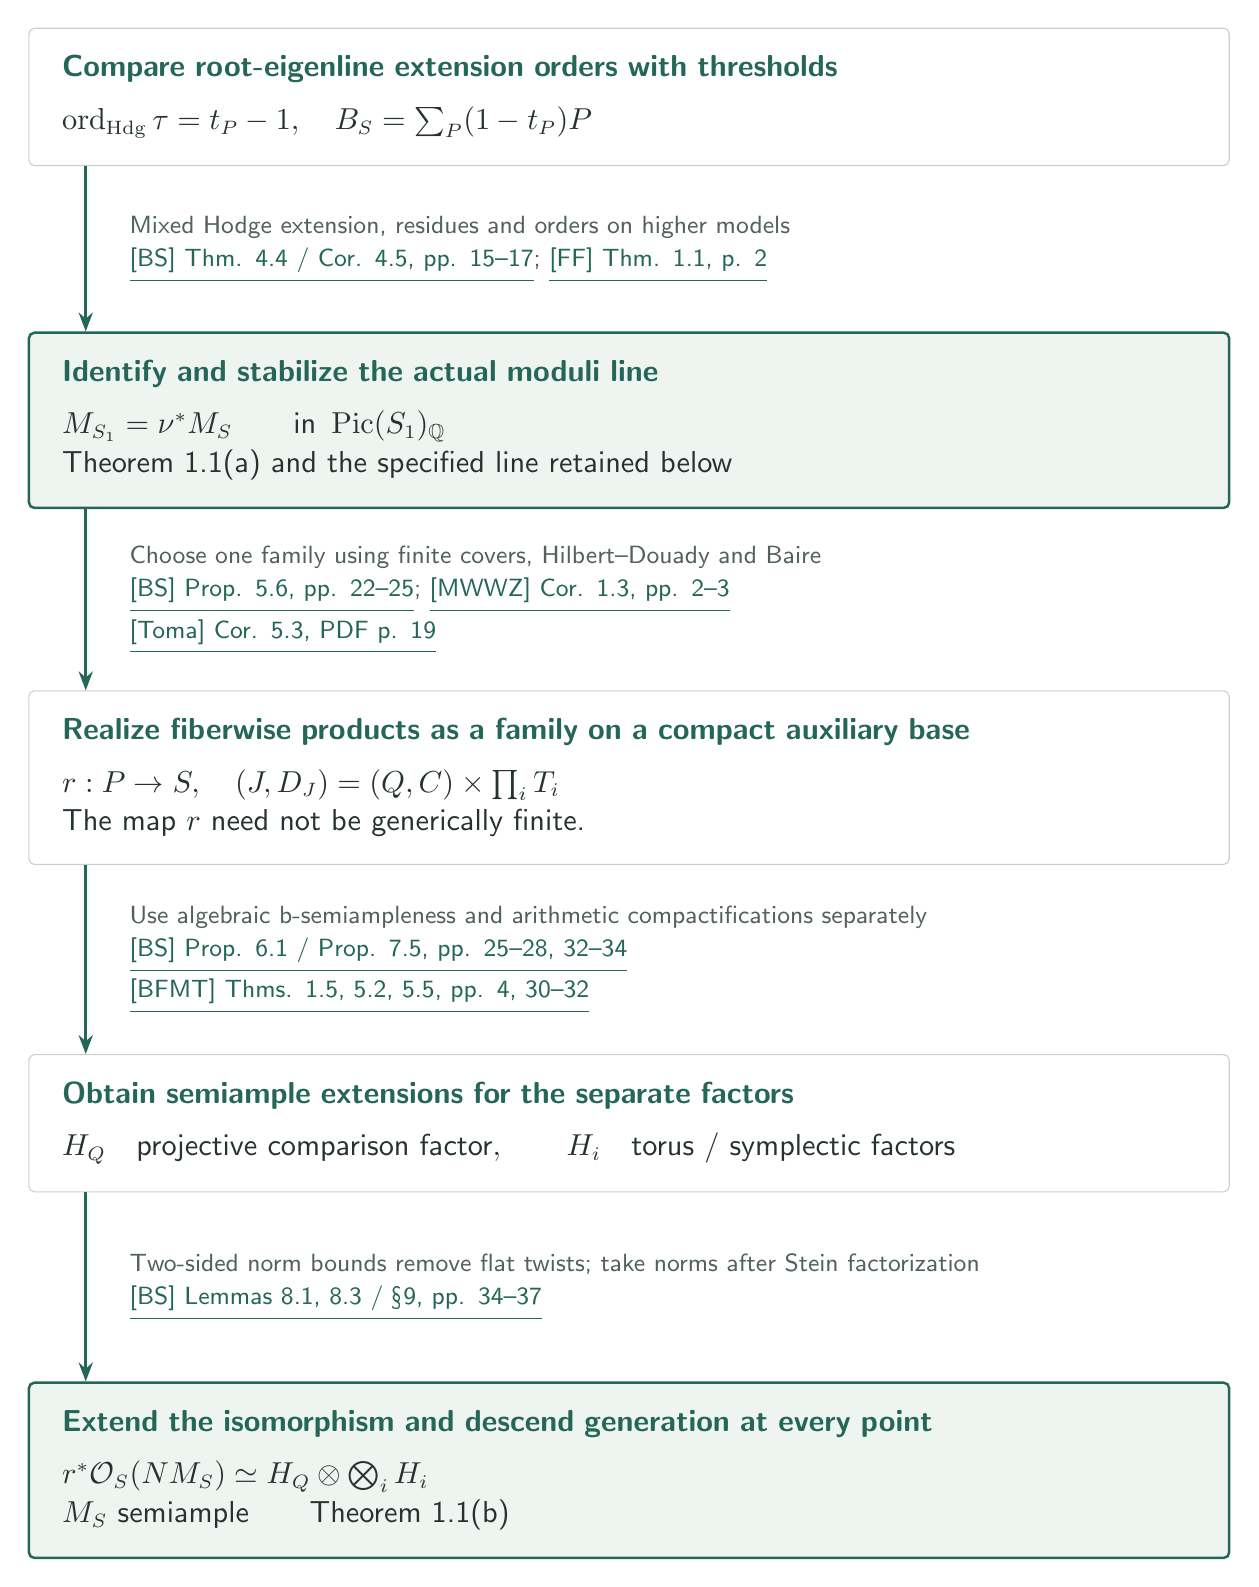
\begin{tikzpicture}
\node[card] (a) {\heading{root eigenlineの延長次数を閾値と比較する}{Compare root-eigenline extension orders with thresholds}
 $\operatorname{ord}_{\mathrm{Hdg}}\tau=t_P-1,\quad B_S=\sum_P(1-t_P)P$};
\node[result,below=2.1cm of a] (b) {\heading{実際のmoduli lineを同定し安定化する}{Identify and stabilize the actual moduli line}
 $M_{S_1}=\nu^*M_S\qquad\text{in }\operatorname{Pic}(S_1)_{\mathbb Q}$\\
 \Tx{Theorem 1.1(a)と、以後も保持する指定されたline}{Theorem 1.1(a) and the specified line retained below}};
\flow{a}{b}{\Tx{混合Hodge延長、留数、全高次モデル上の次数比較}{Mixed Hodge extension, residues and orders on higher models}\\
 \R{BS}{[BS] Thm. 4.4 / Cor. 4.5, pp. 15--17}; \R{FF}{[FF] Thm. 1.1, p. 2}}
\node[card,below=2.3cm of b] (c) {\heading{点ごとの積分解をコンパクトな補助底上の族にする}{Realize fiberwise products as a family on a compact auxiliary base}
 $r:P\to S,\quad (J,D_J)=(Q,C)\times\prod_iT_i$\\
 \Tx{$r$の一般有限性を仮定しない}{The map $r$ need not be generically finite.}};
\flow{b}{c}{\Tx{有限被覆・Hilbert--Douady・Baireで一つの族を選ぶ}{Choose one family using finite covers, Hilbert--Douady and Baire}\\
 \R{BS}{[BS] Prop. 5.6, pp. 22--25}; \R{MWWZ}{[MWWZ] Cor. 1.3, pp. 2--3}\\
 \R{Toma}{[Toma] Cor. 5.3, PDF p. 19}}
\node[card,below=2.4cm of c] (d) {\heading{因子ごとに半豊富な延長を得る}{Obtain semiample extensions for the separate factors}
 $H_Q\quad\Tx{\text{射影的比較因子}}{\text{projective comparison factor}},\qquad
 H_i\quad\Tx{\text{torus・symplectic因子}}{\text{torus / symplectic factors}}$};
\flow{c}{d}{\Tx{代数的b-semiamplenessと算術periodコンパクト化を分けて使う}{Use algebraic b-semiampleness and arithmetic compactifications separately}\\
 \R{BS}{[BS] Prop. 6.1 / Prop. 7.5, pp. 25--28, 32--34}\\
 \R{BFMT}{[BFMT] Thms. 1.5, 5.2, 5.5, pp. 4, 30--32}}
\node[result,below=2.4cm of d] (e) {\heading{同型を延長し、全点での大域生成を降ろす}{Extend the isomorphism and descend generation at every point}
 $r^*\mathcal O_S(NM_S)\simeq H_Q\otimes\bigotimes_i H_i$\\
 $M_S\ \text{semiample}\qquad\text{Theorem 1.1(b)}$};
\flow{d}{e}{\Tx{両側ノルム評価でflat twistを除き、Stein分解後にnormを取る}{Two-sided norm bounds remove flat twists; take norms after Stein factorization}\\
 \R{BS}{[BS] Lemmas 8.1, 8.3 / \S9, pp. 34--37}}
\end{tikzpicture}


\end{document}
